% !TEX root=../../thesis.tex

\section{Prototype functionality} % (fold)
\label{sec:prototype_functionality}
As part of answering the research question, a prototype was developed. In this
section we will describe the functionality in the prototype.\\

The prototype is a map based system that presents the information according to
the needs of the stakeholders, as presented in \Ref{fig:map_prototype}. A
interactive list was implemented, presented in \Ref{fig:stakeholder_selection_list},
which gives the functionality to navigate through the stakeholders hierarchy.
The system aggregates the data according to the current selected stakeholder,
as presented in \Vref{sub:back_end_aggregation}. The visual presentation will 
be adapted to the the areas of responsibility of the current stakeholder, 
which will focus the presentation of the data in the geographical area of the 
stakeholder.

To let the stakeholder be able to select different types of information
according to their need, all types were presented in a list (\Ref{fig:implementation_type_selection}).
The system changes the information presented, when a information type have 
been clicked on.
By letting the user select the information type to present, the system is able
to present the stakeholders need for different information type according to
their requirements. \Ref{fig:crossings_and_speed_restriction_implementation}
shows the presentation of two different types of information.\\

A method to navigate in time were implemented, as the stakeholders have 
different needs for the level of detail in the presentation of data. The time
navigation were implemented as two input boxes, see \Ref{fig:time_selection_implemented}.
The system uses the time interval set by the user to limit the data to be
processed. 

\begin{figure}[!htbp]
	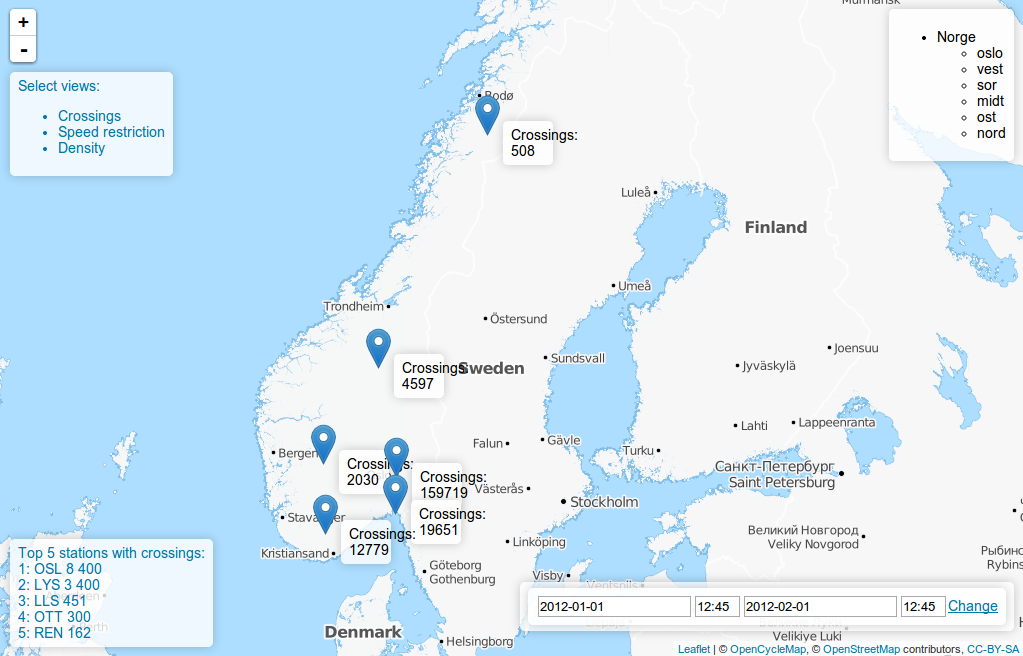
\includegraphics[width=\textwidth,center]{map_prototype.png}
	\caption[Map implementation]{Map implementation}
	\label{fig:map_prototype}
\end{figure}

\begin{figure}[h!tbp]
	\centering
	\begin{subfigure}{0.4\textwidth}
		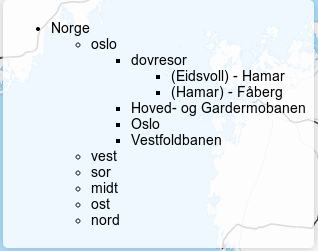
\includegraphics[width=\textwidth]{stakeholder_selection_list.png}
		\caption[Stakeholder selection list]{Stakeholder selection list}
		\label{fig:stakeholder_selection_list}
	\end{subfigure}
	\begin{subfigure}{0.3\textwidth}
		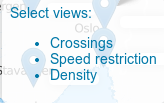
\includegraphics[width=\textwidth]{information_type_selection.png}
		\caption[Information type selection]{Information type selection}
		\label{fig:implementation_type_selection}
	\end{subfigure}
	\caption[Stakeholder selection and Information type]{Stakeholder selection and Information type}
	\label{fig:stakeholder_selection_and_information_type}
\end{figure}

\begin{figure}[h!tbp]
	\centering
	\begin{subfigure}{0.4\textwidth}
		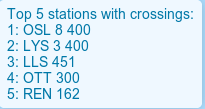
\includegraphics[width=\textwidth]{top5.png}
		\caption[Top 5 list]{Top 5 list}
		\label{fig:top_5_list}
	\end{subfigure}
	\begin{subfigure}{0.6\textwidth}
		
\includegraphics[width=\textwidth]{time_selection_implemented.png}
		\caption[Time selection implementation]{Time selection implementation}
		\label{fig:time_selection_implemented}
	\end{subfigure}
	\caption[Top 5 list and Time selection]{Top 5 list and Time selection}
	\label{fig:Top5_list_and_time_selection}
\end{figure}

\begin{figure}[h!tbp]
	\centering
	\begin{subfigure}{0.6\textwidth}
		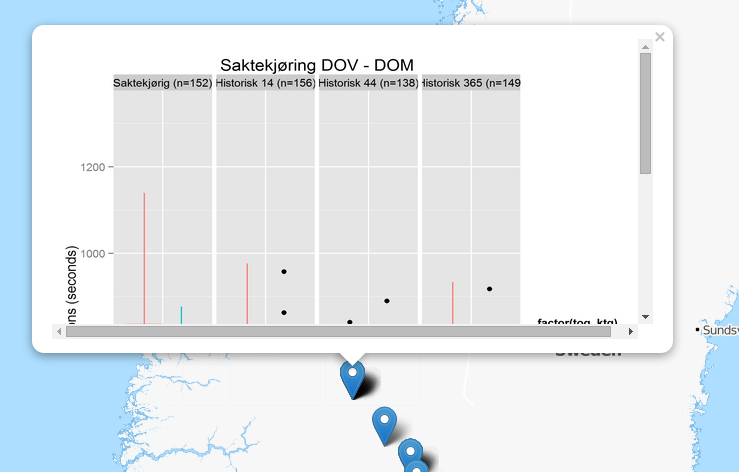
\includegraphics[width=\textwidth]{speed_restriction_presentation.png}
		\caption[Speed restriction presentation]{Speed restriction presentation}
		\label{fig:speed_restriction_presentation}
	\end{subfigure}
	\begin{subfigure}{0.25\textwidth}
		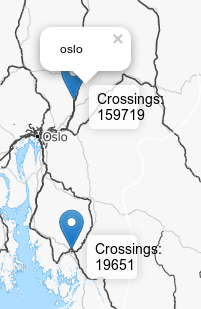
\includegraphics[width=\textwidth]{crossings_presentation.png}
		\caption[Crossings presentation]{Crossings presentation}
		\label{fig:crossings_presentation}
	\end{subfigure}
	\caption[Speed restriction and Crossings implementation]{Speed restriction and Crossings implementation}
	\label{fig:crossings_and_speed_restriction_implementation}
\end{figure}

% section prototype_functionality (end)
